\begin{mdframed}[style=warning]
	\textbf{Conceptos}
		\begin{enumerate}
			\item Si un reloj de péndulo se sube a la cima de una montaña, ¿se adelanta o atrasa? Explique, suponiendo que la marca de hora es correcta a menor altitud.
			\item ¿Qué debe hacerse a la longitud de la cuerda de un péndulo simple para $a)$ duplicar su frecuencia, $b)$ duplicar su periodo, $c)$ duplicar su frecuencia angular?
		\end{enumerate}
\end{mdframed}






\begin{mdframed}[style=warning]
	\begin{ejercicio}
		Un bote esta flotando en un gran contenedor de agua como se ve en la figura \ref{ej4}. El bote está en equilibrio sumergido una distancia $d_o$. Demuestre que si es empujado a una distancia $d$ y se suelta, se inducirá un movimiento armónico. Encuentre su frecuencia de oscilación. Si $d_o = 20cm$, cual es el periodo?
		
		\begin{figure}[H]
			\centering
			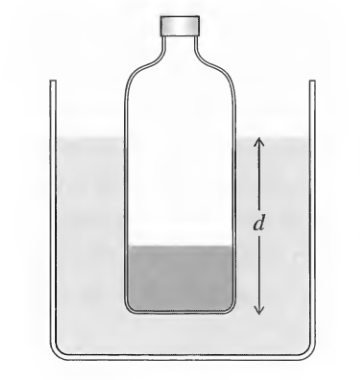
\includegraphics[scale=0.3]{./img/ej4.png}
			\caption{\centering El bote tiene arena para que pueda flotar verticalmente. Esta en equilibrio a una profundidad de $d_o$.}
			\label{ej4}
		\end{figure}
	\end{ejercicio}
\end{mdframed}


























\begin{mdframed}[style=warning]
	\begin{ejercicio}
		Una varilla metálica delgada y uniforme con masa $M$ pivota sin fricción sobre un eje que pasa por su punto medio y es perpendicular a la varilla. Un resorte horizontal con constante de fuerza $k$ se conecta al extremo inferior de la varilla, y el otro extremo del resorte se fija a un soporte rígido. La varilla se desplaza un ángulo pequeño $\theta$ conrespecto a la vertical y se suelta. Demuestre que se mueve en MAS angular y calcule su periodo.
		
		\begin{figure}[H]
			\centering
			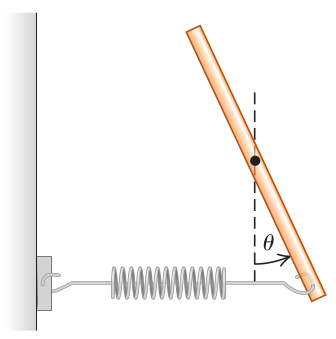
\includegraphics[scale=0.3]{./img/ej1.png}
		\end{figure}
	\end{ejercicio}
\end{mdframed}






















\begin{mdframed}[style=warning]
	\begin{ejercicio}
		Un péndulo de longitud $L$ y masa $M$ tiene un resorte con constante de fuerza $k$ conectado a él a una distancia $h$ bajo su punto de susprensión. Encuentre la frecuencia de vibración del sistema para pequeños valores de la amplitud $\theta$. Suponga que la barra de susprensión vertical de longitud $L$ es rígida, pero ignore su masa.
		
		\begin{figure}[H]
			\centering
			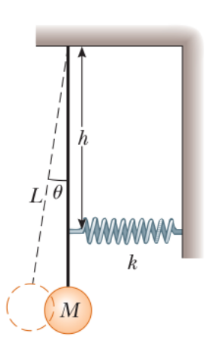
\includegraphics[scale=0.3]{./img/ej2.png}
		\end{figure}
	\end{ejercicio}
\end{mdframed}





















\begin{mdframed}[style=warning]
	\begin{ejercicio}
		Imagine que a través del centro de la Tierra, se cava un hoyo que sale hasta el otro lado y usted, masa $m$, se lanza hacia él. Demuestre que tendrá un movimiento armónico simple si se mueve sin fricción. ¿Cuándo llegará al otro lado de la Tierra?
	\end{ejercicio}
\end{mdframed}







%%%